\documentclass[10pt, landscape]{article}
\usepackage[scaled=0.92]{helvet}
\usepackage{calc}
\usepackage{multicol}
\usepackage{ifthen}
\usepackage[a4paper,margin=3mm]{geometry}
\usepackage{amsmath,amsthm,amsfonts,amssymb}
\usepackage{color,graphicx,overpic}
\usepackage{hyperref}
\usepackage{newtxtext} 
\usepackage{enumitem}
\usepackage[table]{xcolor}
\usepackage{mathtools}
\setlist{nosep}

\usepackage[outputdir=../]{minted} % for code syntax highlighting
\usepackage{mdframed} % framing, backgrounds

% for including images
\graphicspath{ {../images/} }

% Turn off header and footer
\pagestyle{empty}

\newenvironment{tightcenter}{%
  \setlength\topsep{0pt}
  \setlength\parskip{0pt}
  \begin{center}
}{%
  \end{center}
}

% redefine section commands to use less space
\makeatletter
\renewcommand{\section}{\@startsection{section}{1}{0mm}%
                                {-1ex plus -.5ex minus -.2ex}%
                                {0.5ex plus .2ex}%x
                                {\normalfont\large\bfseries}}
\renewcommand{\subsection}{\@startsection{subsection}{2}{0mm}%
                                {-1explus -.5ex minus -.2ex}%
                                {0.5ex plus .2ex}%
                                {\normalfont\normalsize\bfseries}}
\renewcommand{\subsubsection}{\@startsection{subsubsection}{3}{0mm}%
                                {-1ex plus -.5ex minus -.2ex}%
                                {1ex plus .2ex}%
                                {\normalfont\small\bfseries}}%
\renewcommand{\familydefault}{\sfdefault}
\renewcommand\rmdefault{\sfdefault}
%  makes nested numbering (e.g. 1.1.1, 1.1.2, etc)
\renewcommand{\labelenumii}{\theenumii}
\renewcommand{\theenumii}{\theenumi.\arabic{enumii}.}
\renewcommand\labelitemii{•}
\renewcommand\labelitemiii{•}
%  convenient absolute value symbol
\newcommand{\abs}[1]{\vert #1 \vert}
%  convenient floor and ceiling
\newcommand{\floor}[1]{\lfloor #1 \rfloor}
\newcommand{\ceil}[1]{\lceil #1 \rceil}
%  convenient modulo
\newcommand{\Mod}[1]{\ \mathrm{mod}\ #1}
%  for logical not operator, iff symbol, convenient "if/then"
\renewcommand{\lnot}{\mathord{\sim}}
\let\then\rightarrow
\let\Then\Rightarrow
%  vectors
\newcommand{\vv}[1]{\boldsymbol{#1}}
\newcommand{\VV}[1]{\overrightarrow{#1}}
%  column vector
\newcommand{\cvv}[1]{\left(\begin{smallmatrix}#1\end{smallmatrix}\right)}

%  CODE
\newcommand{\code}[1]{\textcolor{myred}{\texttt{#1}}}
\newcommand{\codeb}[1]{\textcolor{myblue}{\texttt{#1}}}
\newcommand{\python}[1]{\mintinline{py}|#1|}
\newcommand{\inline}{\mintinline[fontsize=\normalsize]{text}}
\newcommand\bggreen{\cellcolor{green!10}}

\makeatother
\definecolor{myblue}{cmyk}{1,.72,0,.38}
\definecolor{myred}{cmyk}{0.0, 0.66, 0.30, 0.33}
\everymath\expandafter{\the\everymath \color{myblue}}
% Define BibTeX command
\def\BibTeX{{\rm B\kern-.05em{\sc i\kern-.025em b}\kern-.08em
    T\kern-.1667em\lower.7ex\hbox{E}\kern-.125emX}}

% Don't print section numbers
\setcounter{secnumdepth}{0}

\setlength{\parindent}{0pt}
\setlength{\parskip}{0pt plus 0.5ex}
%% this changes all items (enumerate and itemize)
\setlength{\leftmargini}{0.5cm}
\setlength{\leftmarginii}{0.4cm}
\setlength{\leftmarginiii}{0.5cm}
\setlist[itemize,1]{leftmargin=2mm,labelindent=1mm,labelsep=1mm}
\setlist[itemize,2]{leftmargin=3mm,labelindent=1mm,labelsep=1mm}
\setlist[itemize,3]{leftmargin=3mm,labelindent=1mm,labelsep=1mm}

%My Environments
\newtheorem{example}[section]{Example}
% =============================================================================================================

\begin{document}
\raggedright
\footnotesize
\begin{multicols}{4}


% multicol parameters
% These lengths are set only within the two main columns
\setlength{\columnseprule}{0.25pt}
\setlength{\premulticols}{1pt}
\setlength{\postmulticols}{1pt}
\setlength{\multicolsep}{1pt}
\setlength{\columnsep}{2pt}

\begin{center}
    \fbox{%
        \parbox{0.9\linewidth}{\centering \textcolor{black}{
            {\Large\textbf{CS2109S}}
            \\ \normalsize{AY24/25S2 Midterms}}
            \\ {\footnotesize \textcolor{myblue}{github.com/zeepheru}}
        }%
    }
\end{center}

\begin{center}
    \fbox{%
        \parbox{0.9\linewidth}{\centering \textcolor{black}{
            {\Large\textbf{EXAM INFO}}
            \\ $90$ minutes, $\sim30$ questions
            \\ \textbf{SEAT:} MPSH2A, 82
            }
        }%
    }
\end{center}

\section{INTELLIGENT AGENTS}
\subsection{PEAS}
Performance measure, Environment, Actuators, Sensors

\textbf{Performance Measure} considerations:
\begin{itemize}
    \item What is best for whom? What are we optimizing? What information is available? Any unintended effects? What are the costs?

    \item \textbf{Rational Agent} chooses actions that maximise perf measure.
\end{itemize}
\subsection{Task Environment}
\begin{itemize}
    \item \textbf{Fully} or \textbf{Partially} Observable - can observe complete state of environment?
    \item \textbf{Deterministic} or \textbf{Stochastic} - randomness.
    \item \textbf{Strategic} or \textbf{Dumb} - prescence of other intelligent agents.
    \item \textbf{Episodic} or \textbf{Sequential} - episodic: choice of action in atomic episode depends \textbf{only} on the episode.
    \item \textbf{Static} or \textbf{Dynamic} - whether environment changes while agent is deliberating.
    \item \textbf{Discrete} or \textbf{Continuous} - distinct, clearly defined percepts and actions
    \item \textbf{Single} or \textbf{Multi}-Agent
\end{itemize}

\subsection{Agents}
Completely specified by the agent function.

\textbf{Agent structures}
\begin{itemize}
    \item \textbf{Simple Reflex} Agents - \code{if ... then}
    \item \textbf{Goal-based Agents} - knows what happens if an action is taken, pick based on goal
    \item \textbf{Utility-based} Agents - predicts utility
    \item \textbf{Learning} Agents - performance element
\end{itemize}

\code{Exploration} vs. \codeb{Exploitation}

\section{SEARCH}

\subsection{Problem Formulation}
\begin{itemize}
    \item States, Initial State, Goal State/Test: \code{is\_goal(state)}
    \item Representation Invariant
    \item Actions: $|actions(state)|\leq b$ \codeb{(branching factor)}
    \item Transition Model: \code{new\_state = transition(state, action)}
    \item Action cost function
\end{itemize}

\subsection{Criteria}
\begin{itemize}
    \item Completeness
    \begin{itemize}
        \item Complete $\Leftarrow \forall$ problems, solution exists.
        \item Incomplete $\Leftarrow \exists$ problem, solution \textbf{does not} exists.
    \end{itemize}
    \item Optimal
    \begin{itemize}
        \item Optimal $\Leftarrow \forall$ solution-producing instance, solution is the best.
    \end{itemize}
    \item Optimal and Incomplete: $\exists$ problem with no solution, but all found solutions are optimal.
\end{itemize}

\section{Uninformed Search}

\begin{minted}[tabsize=4]{python}
frontier = Frontier()

frontier.append(Node(initial_state)
while frontier is not empty:
	node = frontier.pop()
	if node.state is goal:
		return solution
		
	for action in actions(node.state):
		next_state = transition(
            node.state, action)
		frontier.add(Node(next_state))
	
return failure    
\end{minted}

\begin{itemize}
    \item \textbf{BFS} - \code{Queue}, explore layer-by-layer
    \item \textbf{UCS} - \code{Pqueue} (by path cost), creates "tiers" based on costs to reach nodes
    \item \textbf{DFS} - \code{Stack}, go deep then backtrack
    \item \textbf{Depth-Limited Search (DLS)} - limit max depth
    \begin{itemize}
        \item Yes DLS (DFS) is not complete and not optimal
        \item "Depth-Limited BFS ensures that we can find the shortest path solution if it exists. The depth limit allows us to terminate in finite time if a solution does not exist."
    \end{itemize}
    \item \textbf{Iterative Deepening Search (IDS)} - DLS with incrementing depth limits
    
\end{itemize}


\section{Informed Search}

\subsection{A* Search}
\begin{equation*}
    f(n) = g(n) + h(n)
\end{equation*}
\begin{itemize}
    \item $g(n)$: cost to reach $n$, $h(n)$: heuristic
    \item Frontier: \code{PQueue( f(n) )}
    \item Complexities are $\exp$
    \item Complete if edges costs are positive and $b$ is finite
    \item Optimality depends on heuristic
\end{itemize}

\subsection{Heuristics}

\begin{itemize}
    \item \textbf{Admissible}
    \begin{itemize}
        \item \textbf{Never over-estimates cost}, it is an optimistic estimate.
        \item Theorem: if $h(n)$ admissible, then A* with visited memory is optimal.
        \item \textbf{Relaxed problem}: fewer restrictions. Optimal solution to a \textbf{relaxed problem} is an admissible heuristic.
    \end{itemize}
    \item \textbf{Consistent}: $\forall$ node $N$ and each successor $P$,
    \begin{itemize}
        \item $h(N) \leq c(N, P) + h(P)$ and $h(G) = 0$
        \item Theorem: if $h(n)$ consistent, then A* with visited memory is optimal.
    \end{itemize}
    \item \textbf{Dominant}: $\forall n, \;h_1(n) \geq h_2(n) \implies h_1 \text{ dominates } h_2$
\end{itemize}

\section{Local Search}

Typically \code{incomplete} and \code{suboptimal}

$\begin{array}{| c | c | c |}
    \hline & \textbf{Perturbatve}  & \textit{Constructive} \\
    \hline \textbf{Search Space} & \text{complete solutions }& \textit{partial solutions} \\
    \hline \textbf{Search step} & \text{modify solution} & \textit{extend solution} \\
    \hline
\end{array}$

\subsection{Problem Formulation}
\begin{itemize}
    \item States: may not map to actual problem state; represent \textbf{potential solutions}
    \item Initial State, \textit{Goal Test (optional)}
    \item Successor Function: generate neighbouring states (candidate solutions)
\end{itemize}

\textbf{Evaluation Function}
\begin{itemize}
    \item Want to \code{minimize} or \codeb{maximize}.
\end{itemize}

\subsection{Hill-Climbing}

\begin{minted}[tabsize=4]{python}
curr_state = initial_state
while True:
    best_successor = 
        """a highest-valued successor 
        state of curr_state"""
    if eval(best_successor) <= eval(curr_state):
        return curr_state
    curr_state = best_successor 
\end{minted}


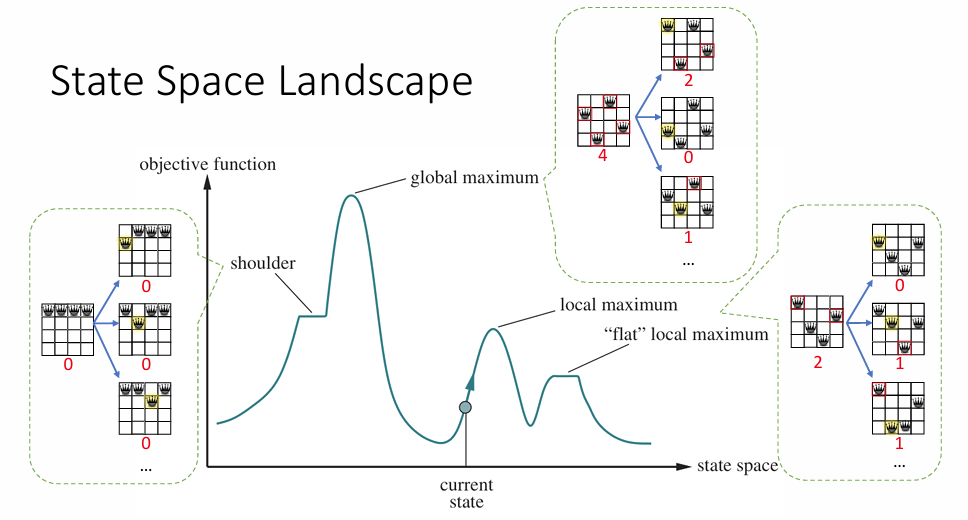
\includegraphics[width=0.8\linewidth]{cs2109s/images/local-search_state_space.png}

\section{Adversarial Search}

\subsection{Problem Formulation}
\begin{itemize}
    \item \textbf{Terminal States}: States of win/lose/draw
    \item \textbf{Utility Function}: Value of state from persp of our agent. \\ Typically need to be computed.
\end{itemize}

\subsection{Minimax}
\code{Two-player zero-sum game}
\begin{itemize}
    \item \textbf{Complete} if tree is finite
    \item \textbf{Optimal} against optimally-playing opponent. \\ Otherwise there will be \textit{faster} strategies.
\end{itemize}


\subsection{Alpha-Beta Pruning}

\begin{minted}[tabsize=4]{python}
def minimax(state):
    # find max value  reachable from this value
    v = max_value(state, -MAX, MAX)
    
    # return a next action that has that state
    return action in expand(state) with value v
        
def max_value(state, a, b):
    if is_terminal(state): 
        return utility(state)
    v = -MAX
    
    # iterate through next states
    for next_state in expand(state):
        v = max(v, min_value(next_state))
        a = max(a, v)
        if v >= b: return v
    return v # max value from current state

def min_value(state, a, b):
    if is_terminal(state): 
		    return utility(state)
    v = MAX
    for next_state in expand(state):
        v = min(v, max_value(next_state))
        a = min(b, v)
        if v <= a: return v
    return v # min value from current state
\end{minted}

Good move ordering improves pruning effectiveness.

\subsection{Cutoff}

Imploying a \code{cutoff} strategy: halt search halfway and estimate value of midgame states using an \textbf{evaluation function}.

Better handles large/infinite game trees.

\section{MACHINE LEARNING}
\begin{itemize}
    \item \textbf{Unsupervised} Learning: \code{Unlabeled} data, find patterns/structure
    \item \textbf{Supervised} Learning: \codeb{Labeled} data, learns mapping
    \begin{itemize}
        \item \textbf{Classification}: Predict discrete label or category
        \item \textbf{Regression}: Predict continuous numerical value
    \end{itemize}
\end{itemize}
Dataset $D = \left\{ (x^{(1)}, y^{(1)}), (x^{(2)}, y^{(2)}), \dots, (x^{(n)}, y^{(n)})\right\}$

True data generating function $f^*(x)$

\textbf{Hypothesis class} $H$ Set of all possible models/functions $h:X\to Y$

\subsection{Performance Measure}
\textbf{Regression}
\begin{align*}
    MSE & = \frac{1}{N}\sum^N_{i=1} \left(\hat{y}^{(i)} - y^{(i)}\right)^2 \\
    MAE & = \frac{1}{N}\sum^N_{i=1} \left|\hat{y}^{(i)} - y^{(i)}\right|
\end{align*}
\textbf{Classification}
\begin{align*}
    Accuracy = \frac{1}{N} \sum^N_{i=1} \mathbf{1}_{\hat{y}^{(i)} = y^{(i)}}
\end{align*}

\begin{center}
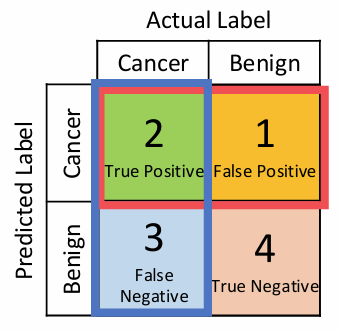
\includegraphics[width=0.6\linewidth]{cs2109s/images/confusion-matrix.png}
\end{center}


\begin{itemize}
    \item \textbf{Accuracy}: ${TP+TN}/total$
    \item \textcolor{myred}{\textbf{Precision}: $TP / (TP + FP)$
    \\ Number of correct out of predicted positives.}
    
    \item \textcolor{myblue}{\textbf{Recall}: $TP / (TP+FN)$
    \\ Number predicted out of \textbf{actual} positives.}
   
    \item \textbf{F1 Score}: $2 \cdot (1/P + 1/R)^{-1}$
\end{itemize}

\section{Decision Trees}
Given $n$ boolean attributes, $2^{2^n}$ distinct trees.

\begin{center}
\textbf{Entropy}:
\begin{align*}
    I(P(v_1) \dots P(v_k)) = -\sum^k_{i=1} P(v_i) \log_2P(v_i)
\end{align*} 
\textbf{Information Gain}: \\
$I$ before dividing - weighted mean $I$ after dividing
\begin{align*}
    remainder(A) = \sum^v_{i=1} \frac{p_i+n_i}{p+n}I\left( \frac{p_i}{p_i+n_i}, \frac{n_i}{p_i+n_i}\right)\\
    IG(A) = I\left( \frac{p_i}{p_i+n_i}, \frac{n_i}{p_i+n_i}\right) - remainder(A)
\end{align*}

\end{center}

\subsection{Decision Tree Learning}

Greedy, top-down, recursive.

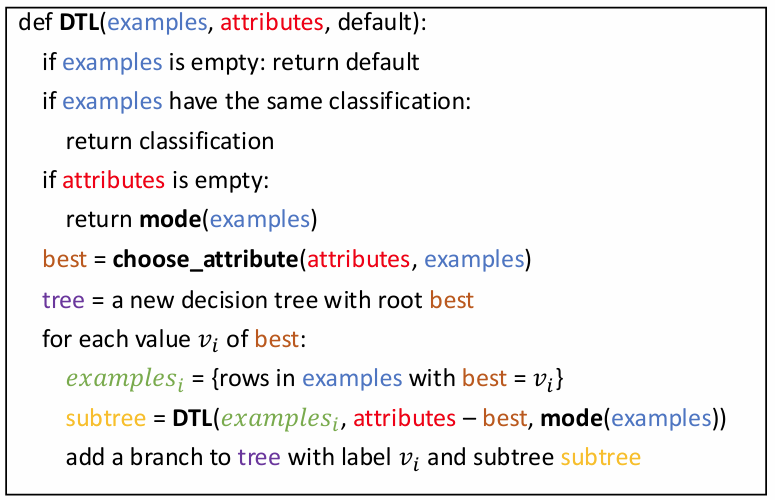
\includegraphics[width=0.9\linewidth]{cs2109s/images/dtl.png}

Decision trees can have issues of \textbf{overfitting} when generalized to new test data.

\textbf{Occam's Razo}r: prefer \textbf{short/simple} hypotheses over \textbf{long/complex}. Less likely to be concidences.

\textbf{Pruning}
\begin{itemize}
    \item \textbf{Min-sample leaf}: Minimum threshold required to be in a leaf node. \\If splitting creates a leaf with nodes $<$ \codeb{}{threshold}, do not split.
    \item \textbf{Max-depth}: Note that depth is is of path from \code{root} to \code{leaf}
\end{itemize}

\textbf{Data Preprocessing}
\begin{itemize}
    \item Partition continuous values (binning)
    \item Deal with missing values: assign common value, drop attribute, drop rows...
\end{itemize}


\section{LINEAR Regression}
Features $x^{(i)} \in \mathbb{R}^d$; target $y^{(i)}\in \mathbb{R}$

\textbf{Linear model}: 
\begin{align*}
h_w(x) = w_0(x_0:1) + w_1x_1 + \dots + w_dx_d = w^Tx
\end{align*}
\textbf{Feature Transformations}
\begin{itemize}
    \item \textbf{Feature Engineering}
    \begin{itemize}
        \item Add a new feature: $z=x^k, z=\log(x), z=e^x$
    \end{itemize}
    \item \textbf{Feature Scaling}
    \begin{itemize}
        \item Min-max scaling: $z_i = \frac{x_i - \min(x_i)}{\max(x_i)-\min(x_i)}$ \\
        This one is to $[0,1]$
        \item Standardization: $z_i = \frac{x_i-\mu_i}{\sigma_i}$
    \end{itemize}
\end{itemize}

\textbf{Loss: MSE}

\begin{align*}
    J_{MSE}(w) = \frac{1}{2N}\sum^N_{i=1} \left(h_w(x^{(i)})-y^{(i)}\right)^2
\end{align*}

\subsection{Normal Equation}
\begin{align*}
    w = (X^TX)^{-1}X^TY
\end{align*}
\begin{itemize}
    \item Slow, inverting requires $O(d^3)$
    \item $X^TX$ needs to be \code{invertible}.
\end{itemize}

\subsection{Gradient Descent}
\begin{align*}
    w_j \stackrel{update}\longleftarrow w_j - \gamma \frac{\partial J(w_0, w_1\dots)}{ \partial w_j}
\end{align*}

Learning rate $\gamma ? 0$, a hyperparameter.

\vspace{2pt}
\textbf{Theorem}: A \code{convex} function has a single global minimum.\\
\textbf{Theorem}: MSE loss function is \code{convex} for linear and polynomial regression.
\vspace{2pt}

To deal with differently-scaled features:
\begin{itemize}
    \item Normalize/Standardize \textit{(or other scaling)}
    \item This can actually make GD \code{faster}.
    \item Different learning rate $\gamma_i$ for each weight.
\end{itemize}


\textbf{Variants}
\begin{itemize}
    \item Introduce \code{randomness}, may escape local minima
    \item \textbf{Mini-batch}: Consider subset of training data at a time.
    \item \textbf{Stochastic (SGD}): Select \textbf{one} random data point at a time.
\end{itemize}

\section{LOGISTIC Regression}
target $y \in \{0,1\}$

\vspace{6pt}
\textbf{Sigmoid/Logistic Function}
\begin{align*}
    \sigma(x) = \frac{1}{1+e^{-x}} \;\bigg|\; \sigma'(x) = \sigma(x)(1-\sigma(x))
\end{align*}


\begin{align*}
    h_w(x) = \sigma(w_0x_0+w_1x_1+\dots +w_dx_d) = \sigma(w^Tx)
\end{align*}
Then compare against \code{decision threshold}.

\textbf{Decision boundary}: separates classes in feature space.

\vspace{6pt}
\textbf{Non-linearly separable}: use non-linear \textbf{feature transformations}, 
e.g. scale to $[-1,1]$, then $x^2$.

\subsection{Loss: BCE}
True value $y$, prediction $\hat y$:
\begin{align*}
    BCE(y, \hat y)= -y \log (\hat y) - (1-y)\log(1-\hat y)\\
    J_{BCE}(w) = \frac{1}{N}\sum^N_{i=1}BCE \left( y^{(i)}, h_w(x^{(i)})\right)
\end{align*}

\vspace{2pt}
\textbf{Theorem}: BCE loss function is \code{convex} for logistic regression.
\vspace{2pt}

\subsection{Multi-class}
target $y \in \{0,1,2, \dots,C\}$

\textbf{One-vs-one}
\begin{itemize}
    \item Separate classifier for every pair.
    \item Class with most votes selected.
\end{itemize}
\textbf{One-vs-rest}
\begin{itemize}
    \item Separate classifier for each class against \textbf{all other} classes.
    \item Class with highest probability (confidence score) selected.
\end{itemize}


\section{Supervised Learning ++}

\subsection{Dataset}
\textbf{Quality}
\begin{itemize}
    \item relevance, noise, balance (classification)
\end{itemize}

\textbf{Quantity}: more usually $\to$ better, but containing \textbf{all} is simply \code{memorization}.

\subsection{Model Complexity}
Size and expressiveness. e.g. \code{Polynomial} higher complexity than \codeb{linear}.

\begin{itemize}
    \item \codeb{Simple model} good enough for simple truth, few data points needed
    \\ \textit{high bias, low variance}
    \item \code{Complex model} overfits if \textbf{few} data points given
    \\ \textit{low bias, high variance}
    \item \textbf{Bias}: Dependency to fit what it's capable of, \code{complex model} can fit data well $\to$ \textbf{low bias}.
    \item \textbf{Variance}: How much model changes as \textbf{number of data points} changes.
\end{itemize}

\subsection{Hyperparameters}
Predefined and adjusted manually. By comparison \textbf{parameters}, e.g. weights, are learned during training.
\begin{itemize}
    \item learning rate, feature transformations, batch size/iterations in mini-batch
\end{itemize}

\textbf{Hyperparmater Tuning}
\begin{itemize}
    \item Grid Search (exhaustive search): trying all possible combinations
    \item Random Search: randomly sampling rates and Hyperparameters
    \item Local Search: e.g. Hill climb
\end{itemize}

\section{MISC}
$$\log_b(a) = \frac{\log_x(a)}{\log_x(b)}$$


\end{multicols}

% =============================================================================================================




% \section{FIXXXXXXXXX}
\begin{minipage}{0.4\linewidth} 


    $\begin{array}{| c | c | c | c | c |}
        \hline\textbf{Search} & \textbf{Time} & \textbf{Space} & \textbf{Complete} & \textbf{Optimal} 
        \\\hline\text{BFS} & \exp & \exp & \checkmark & \checkmark
        \\\hline\text{UCS} & \exp & \exp & \checkmark & \checkmark
        \\\hline\text{DFS} & \exp & m^k & \times & \times
        \\\hline\text{DLS (DFS)} & \exp & \exp & \times & \times
        \\\hline\text{IDS} & \exp & m^k & \checkmark & \checkmark
        \\\hline\text{A*} & \exp & \exp & \checkmark^* & \textit{depends}
        \\\hline\text{Minimax} & \exp, O(b^m) & m^k & \checkmark^* & \checkmark^*
        \\\hline
    \end{array} 
    $\

    Time complexity: nodes generated; Space complexity: size of frontier.


    
\end{minipage}%
\begin{minipage}{0.6\linewidth}   
    \begin{multicols}{2}
        More text.
    \end{multicols}
\end{minipage}

\end{document}